%********************************************************************
% Appendix
%*******************************************************
% If problems with the headers: get headings in appendix etc. right
%\markboth{\spacedlowsmallcaps{Appendix}}{\spacedlowsmallcaps{Appendix}}



\chapter{Test: APDU Commands exchanged}\label{ch:resultsdiagrams}


In this appendix we provide 3 sequence diagrams highlighting the APDU Commands exchanged during our testbed. 


The first one is the setup of the IoT smart card, storing the system parameters needed to work in the deployed P2ABCE system. The first Command is called \texttt{isAndroid} because the \texttt{HardwareSmartcard} class distinguishes Android phones acting as smart cards from MULTOS smart cards, in order to use Extended APDUs. Then configures the smart card, setting the PIN (``\texttt{1234}'' by default) and PUK. Finally, it copies the cryptographic system parameters to the smart card with multiple \texttt{SET} instructions.

The second image shows the issuance of the credential, divided in the three REST calls needed during the delegation. If we recall Idemix's issuance protocol, the User performed, during his first step, an exponentiation with his secret key and a ZKP, which can be identified by the \texttt{COMMITMENT} and \texttt{ISSUANCE RESPONSE} commands. During the second step, the User only has to verify the Issuer's ZKP and store the credential if the signature is valid. Because the P2ABC Engine can perform Verification of ZKP without the need of secret keys stored in the smart card, the APDU Commands in this phase are only for storing the credential information inside the IoT smart card's BLOB\footnote{\textbf{B}inary \textbf{L}arge \textbf{Ob}jects} database, with the \texttt{STORE BLOB} instruction. 


The last diagram represents the proving for the Presentation Policy received from a Verifier, using two REST calls. During the first REST call, the Service stores data for the proving in the smart card, but before starting the proving itself, the device must choose an identity for the proving. This is done with the Identity Service, that in the PoC chooses the first identity available. After this, the second REST call starts the proving, creating the \textit{commitment} and \textit{responses} that integrate any ZKP, and depends on the device's secret keys\footnote{We, again, refer the reader who wants to know more about ZKPs to \citep{tfgmates}.}.


\begin{figure}[bth]
	\begin{center}
		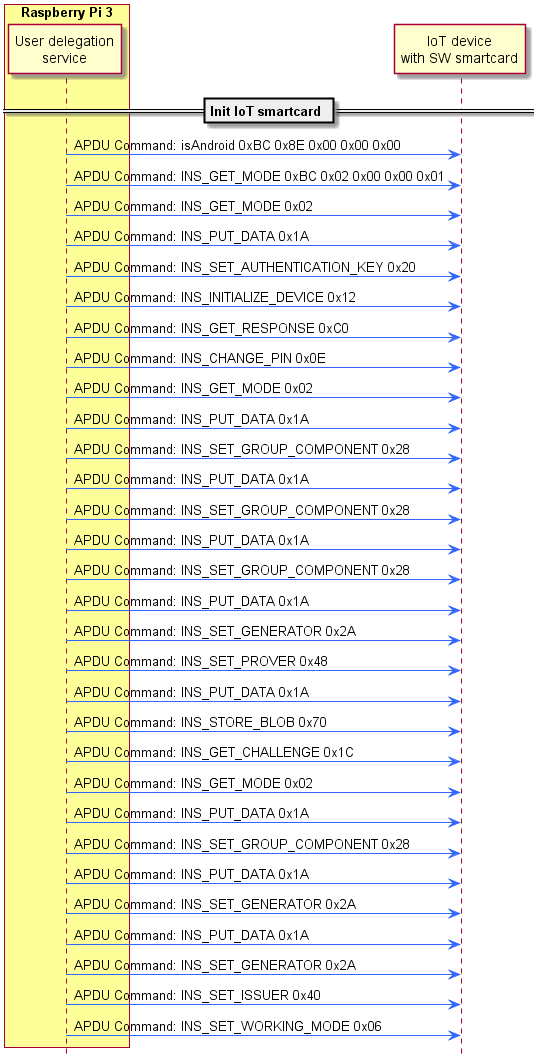
\includegraphics[width=0.9\linewidth]{gfx/UML/APDUsInitIoTSC}
	\end{center}
	\caption{Init IoT Smart Card APDU Commands exchanged.}
	\label{fig:APDUsInitIoTSC}
\end{figure}

\begin{figure}[bth]
	\begin{center}
		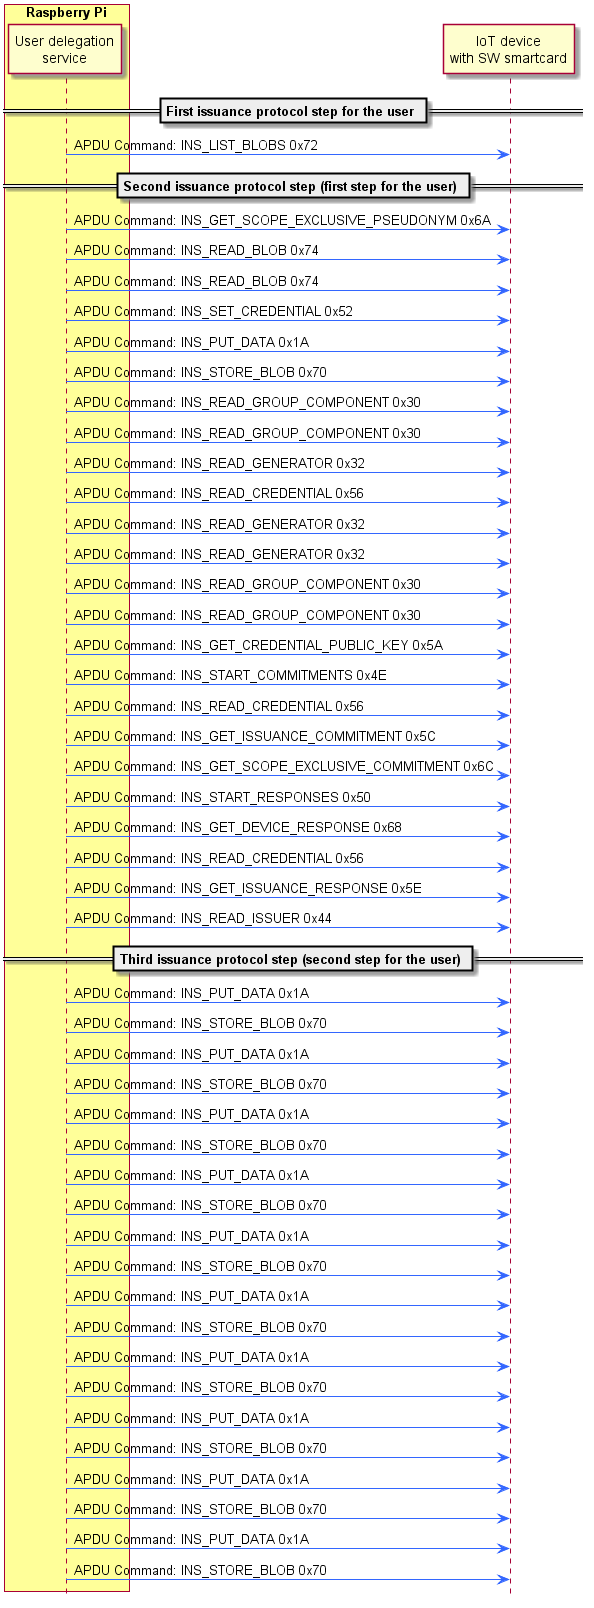
\includegraphics[width=0.78\linewidth]{gfx/UML/IssuanceAPDUs}
	\end{center}
	\caption{Issuance APDU Commands.}
	\label{fig:IssuanceAPDUs}
\end{figure}

\begin{figure}[bth]
	\begin{center}
		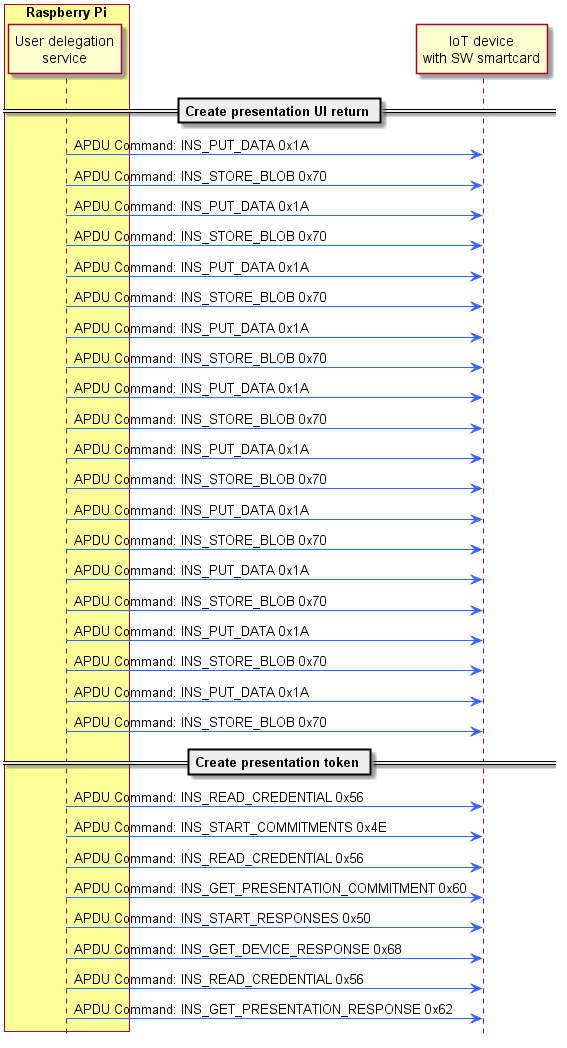
\includegraphics[width=\linewidth]{gfx/UML/APDUsProving}
	\end{center}
	\caption{Proving APDU Commands.}
	\label{fig:APDUsProving}
\end{figure}



\chapter{Paper proposal for JCR Magazine}\label{ch:JCR}

a


\chapter{Project's code structure}\label{ch:code}

Given the size of the project, we identify four main directory structures to arrange the code.


First, the Dockerfiles, scripts that automatize the creation of Docker images. These images are like virtual machine snapshots, although Docker is not a virtualization system, and we use the images to create containers, that are like new virtual machines started from the snapshots. We use two Dockerfiles, one for the P2ABCE compilation environment, with Java and Maven, and another one for building the Omega2 binaries, using the LEDE SDK.


\dirtree{%
	.1 Docker/. 
	.2 P2ABCE/. 
	.3 Dockerfile. 
	.3 idemix-3.0.36-binaries/. 
	.2 LEDE SDK/. 
	.3 Dockerfile. 
}

\hfil

The original P2ABCE project is of considerable size, but we list here the most interesting directories that we had to modify to make the project compatible with IoT smart cards.

\hfil

\dirtree{%
	.1 P2ABCE/. 
	.2 Code/. 
	.3 core-abce/. 
	.4 abce-components/. 
	.5 src/main/java/eu/abc4trust/smartcard/. 
	.6 IoTsmartcardio/.
	.7 util/. 
	.8 IoTsmartcardConnection.java.  
	.7 IoTCard.java. 
	.7 IoTCardChannel.java. 
	.7 IoTCardTerminal.java. 
	.6 HardwareSmartcard.java. 
	.6 SoftwareSmartcard.java. 
	.4 abce-services/. 
	.5 src/main/java/eu/abc4trust/services/. 
	.6 UserService.java. 
	.6 VerificationService.java. 
	.6 IssuanceService.java. 
}



\hfil

The IoT smart card toolkit is the core of this project. Managed with CMake, we see the \texttt{CMakeLists.txt} files, including the \texttt{Toolchain-omega2-mipsel.cmake} file with the cross-compiler information. We divide the project between the \textit{source} C files, and the header C files. Inside these directories, the organization is as stated in the implementation chapter: \textit{core} or \textit{common}, \textit{util interfaces} and \textit{external utilities}.

\hfil

\dirtree{%
	.1 p2abce\_iot\_toolkit/. 
	.2 CMakeLists.txt. 
	.2 Toolchain-omega2-mipsel.cmake. 
	.2 util\_sc\_tests/. 
	.2 util\_sc/. 
	.3 CMakeLists.txt. 
	.3 BIOSC.c. 
	.3 p2abc\_iot\_toolkit\_src/. 
	.4 smartcard\_common/. 
	.5 APDU\_handler.c. 
	.5 global\_vars.c. 
	.5 m\_adapted\_API.c. 
	.5 subroutines.c. 
	.4 smartcard\_external\_utilities/. 
	.5 cJSON.c. 
	.4 smartcard\_utils\_interface/. 
	.5 APDU\_IO\_util.c. 
	.5 arithmetic\_util.c. 
	.5 crypto\_util.c. 
	.5 serialize\_util.c. 
	.5 system\_funcs.c. 
	.3 p2abc\_iot\_toolkit\_include/. 
	.4 error\_codes.h. 
	.4 macrologger.h. 
	.4 smartcard\_common/. 
	.5 APDU\_handler.h. 
	.5 APDU\_types.h. 
	.5 abc4T\_types.h. 
	.5 defs\_consts.h. 
	.5 defs\_errs.h. 
	.5 defs\_ins.h. 
	.5 defs\_types.h. 
	.5 global\_vars.h. 
	.5 m\_adapted\_API.h. 
	.5 subroutines.h. 
	.4 smartcard\_external\_utilities/. 
	.5 base64.h. 
	.5 cJSON.h. 
	.4 smartcard\_utils\_interface/. 
	.5 APDU\_IO\_util.h. 
	.5 arithmetic\_util.h. 
	.5 crypto\_util.h. 
	.5 serialize\_util.h. 
	.5 system\_funcs.h. 
}


\hfil

Finally, the test scripts, including a Python file to test the BIOSC protocol, a directory with the testbed scripts (one file to orchestrate every device from one terminal), and a more didactic version with a script per device.

\hfil

\dirtree{%
	.1 scripts/. 
	.2 testBIOSC.py. 
	.2 tests/\DTcomment{One test script}. 
	.3 setupTest.sh. 
	.3 testNoIoT.sh. 
	.3 IoTtest.sh. 
	.2 distributed-PoC/\DTcomment{Distributed test}. 
	.3 Omega2/. 
	.3 RaspberryPi3/. 
	.3 ThirdPartyServer/. 
}